\chapter{Obrazové přílohy}

\begin{figure}[h]
    \centering
    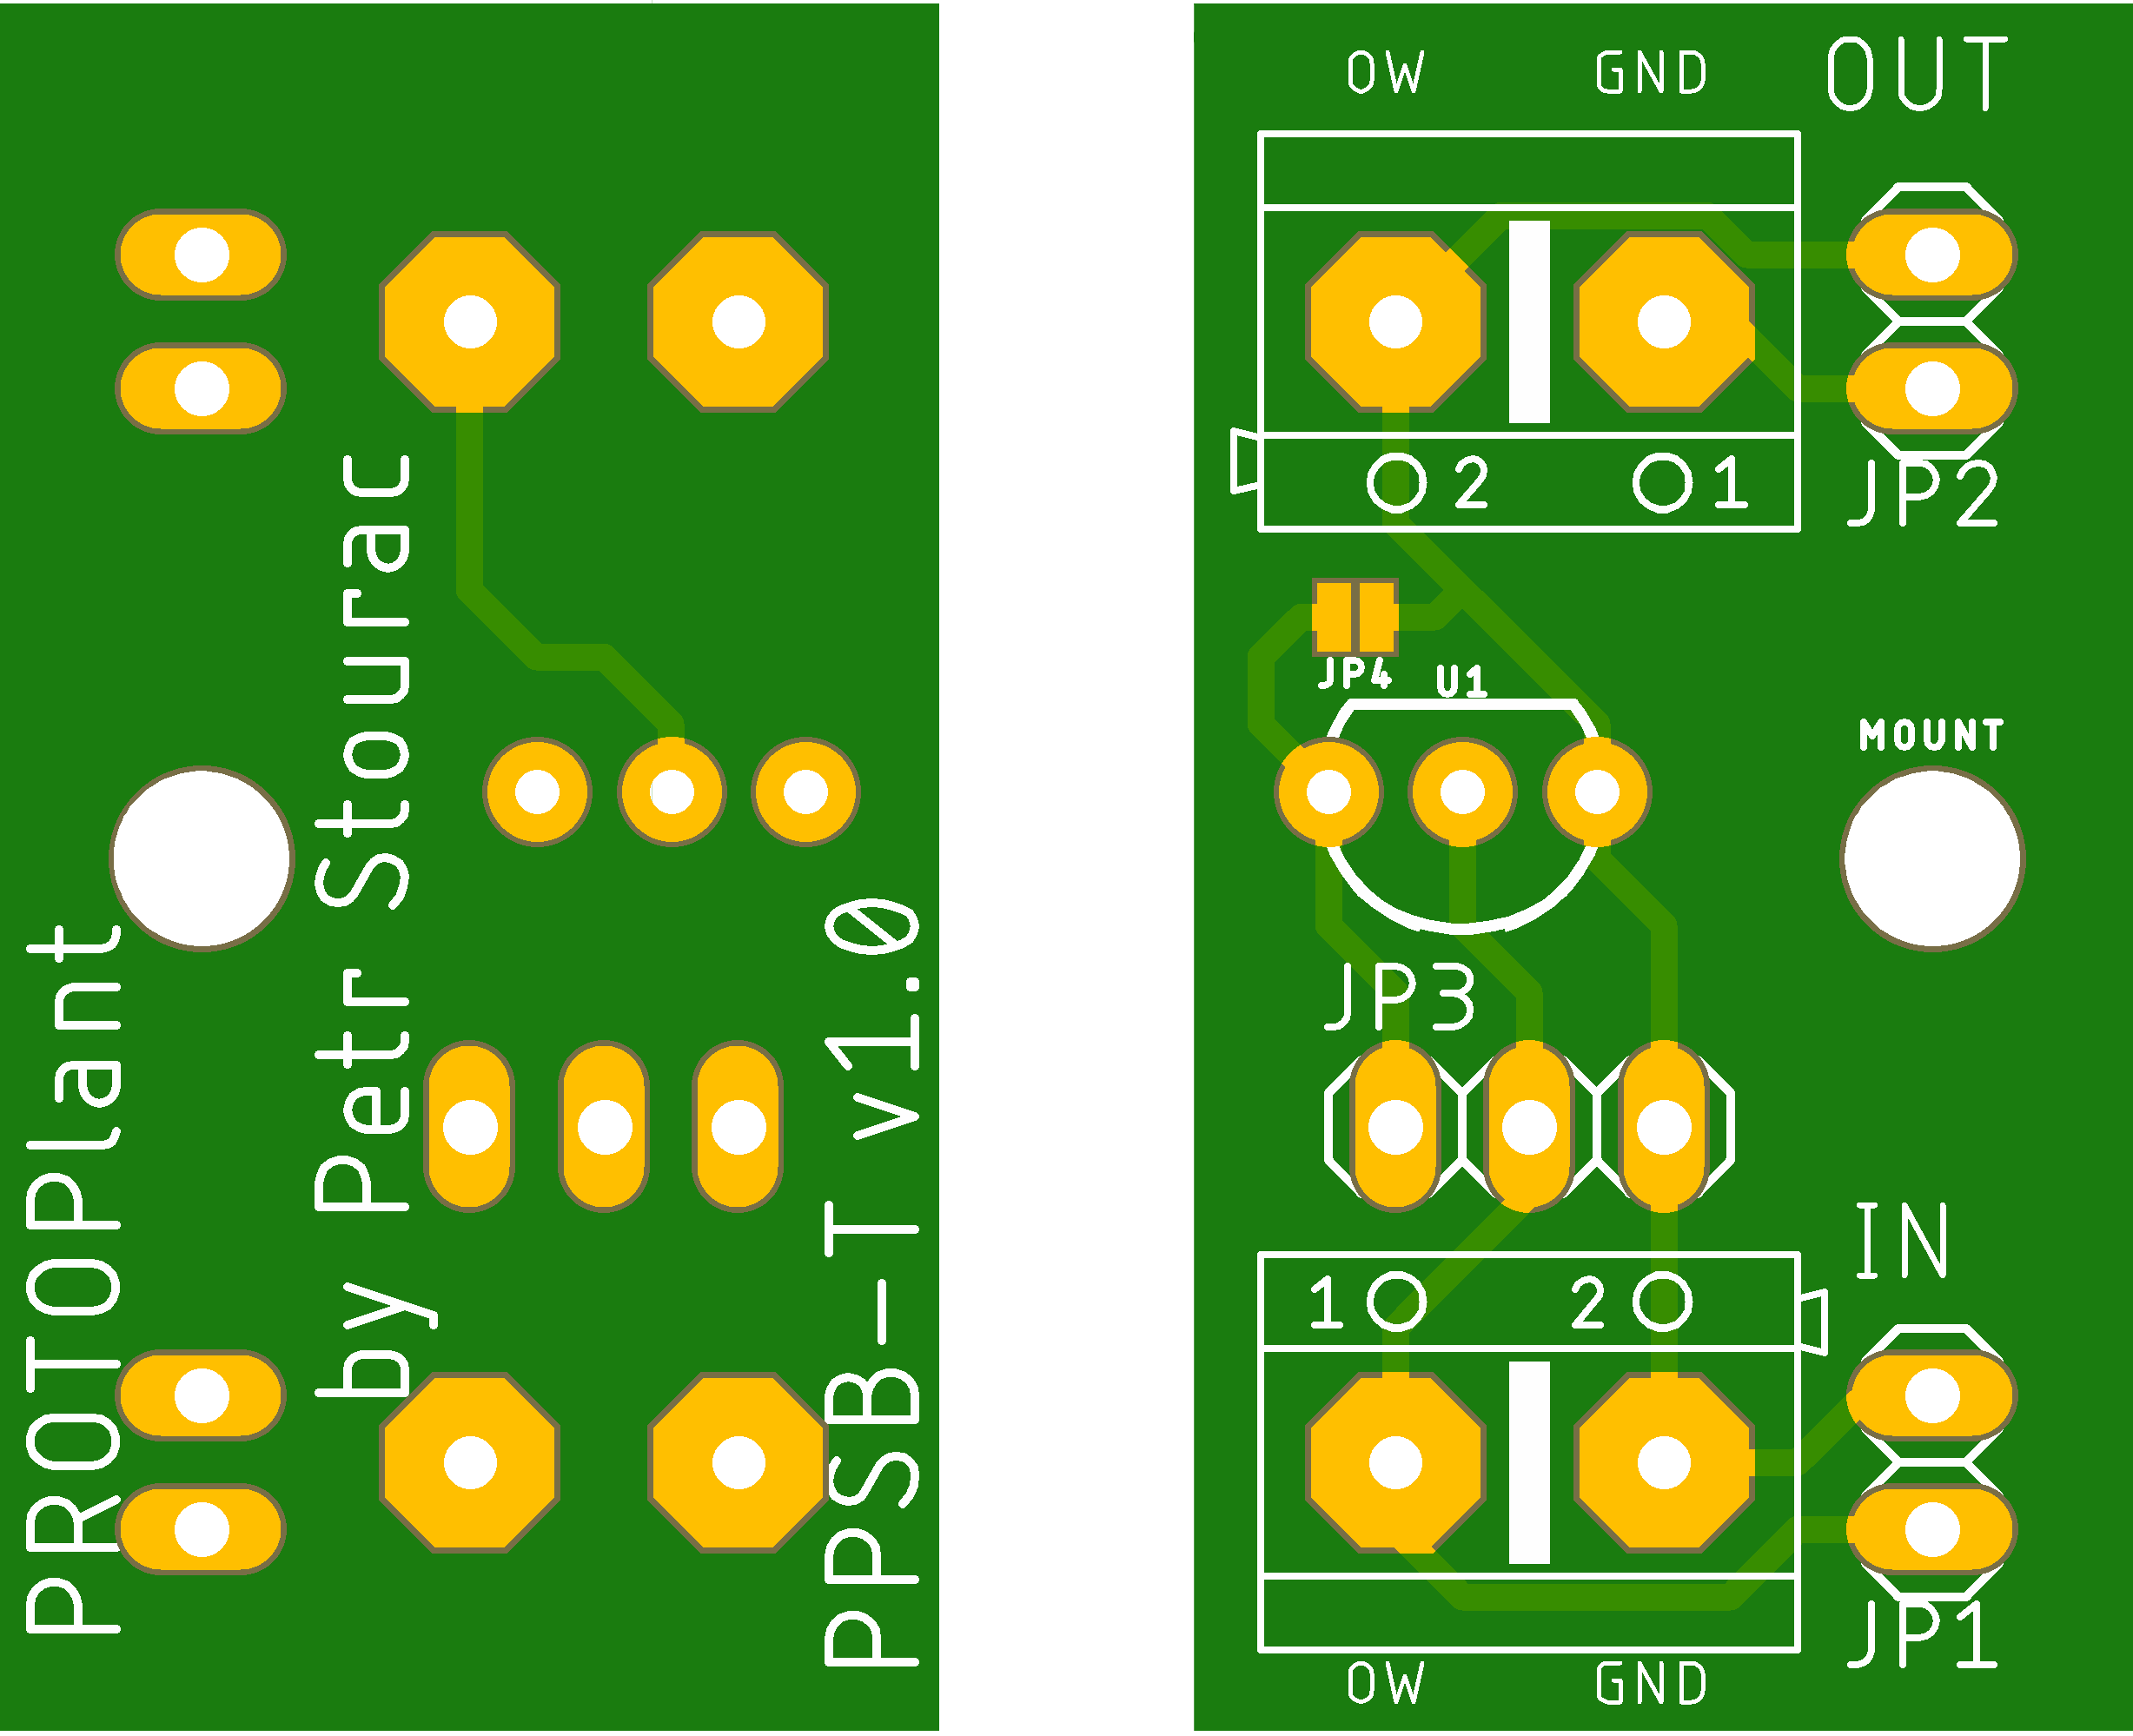
\includegraphics[width=0.85\textwidth]{img/HARDWARE/PPSB-T_BOTH.png}
    \caption{Vizualizace PPSB-T (horní strana vpravo, dolní vlevo).}
    \label{fig:PPSB-T_VISUAL}
\end{figure}

\begin{figure}[h]
    \centering
    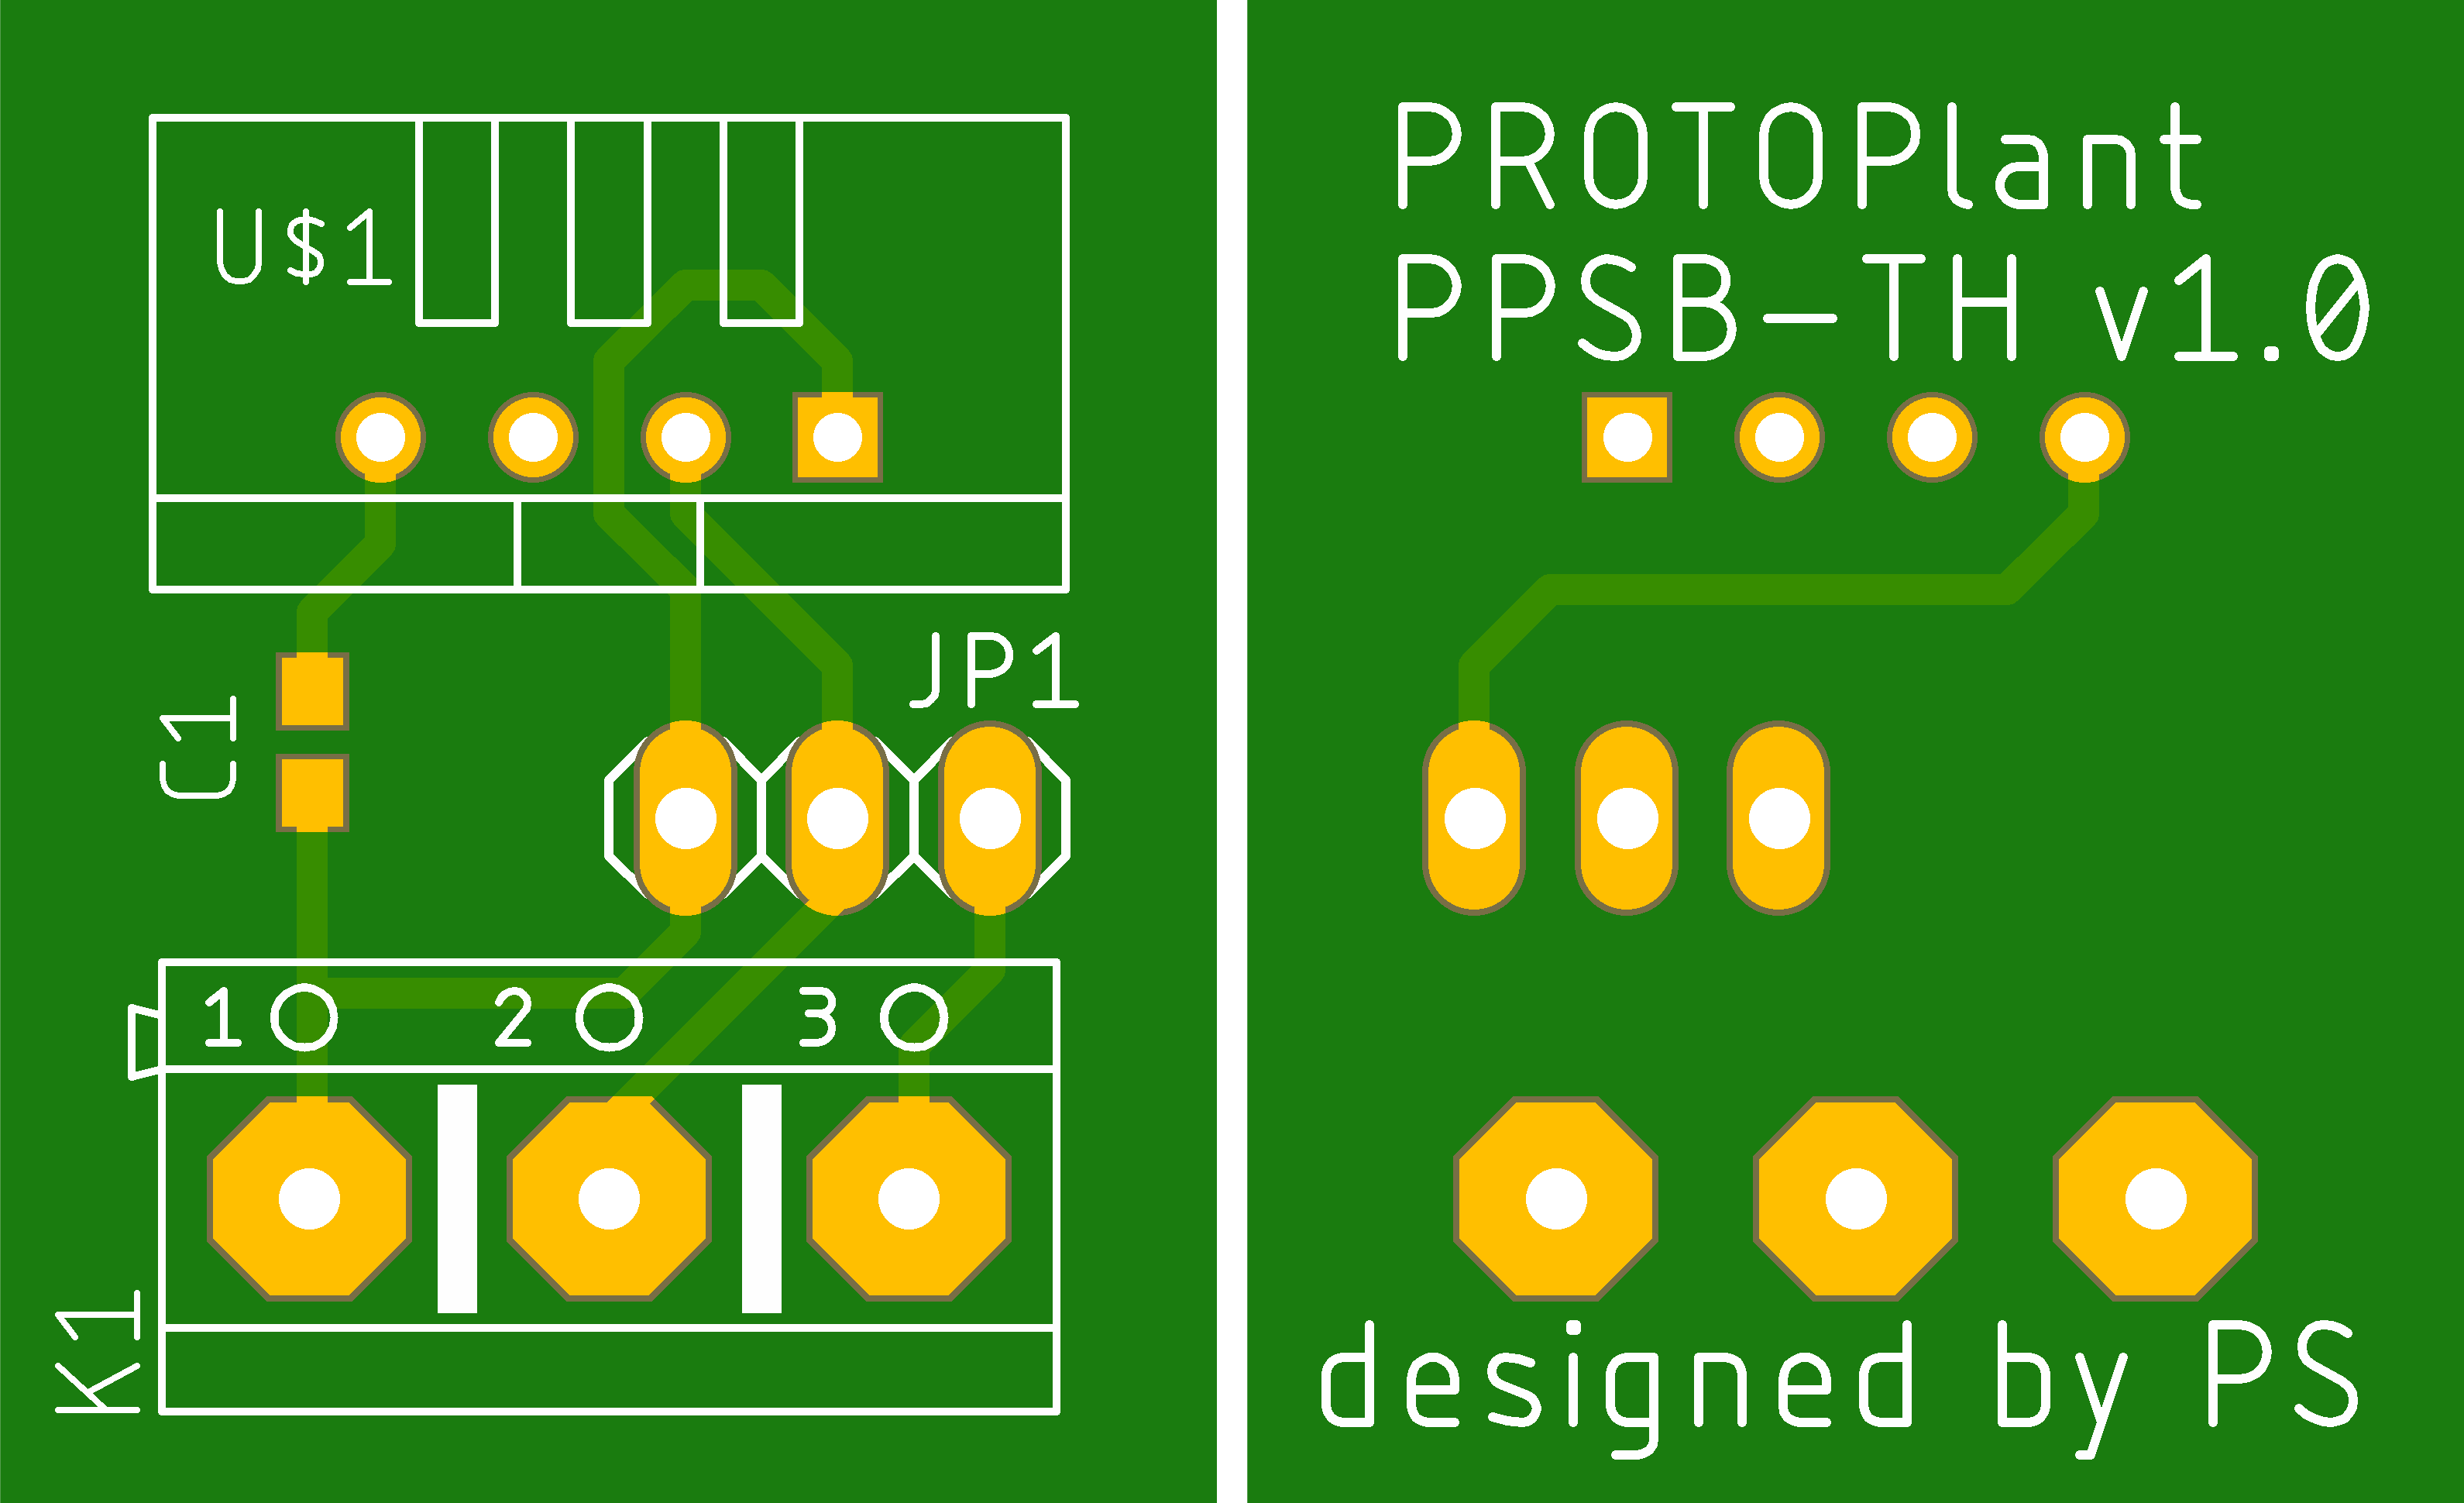
\includegraphics[width=0.85\textwidth]{img/HARDWARE/PPSB-TH_BOTH.png}
    \caption{Vizualizace desky PPSB-TH (horní strana vlevo, dolní vpravo).}
    \label{fig:PPSB-TH_VISUAL}
\end{figure}

\begin{figure}[htbp]
    \centering
    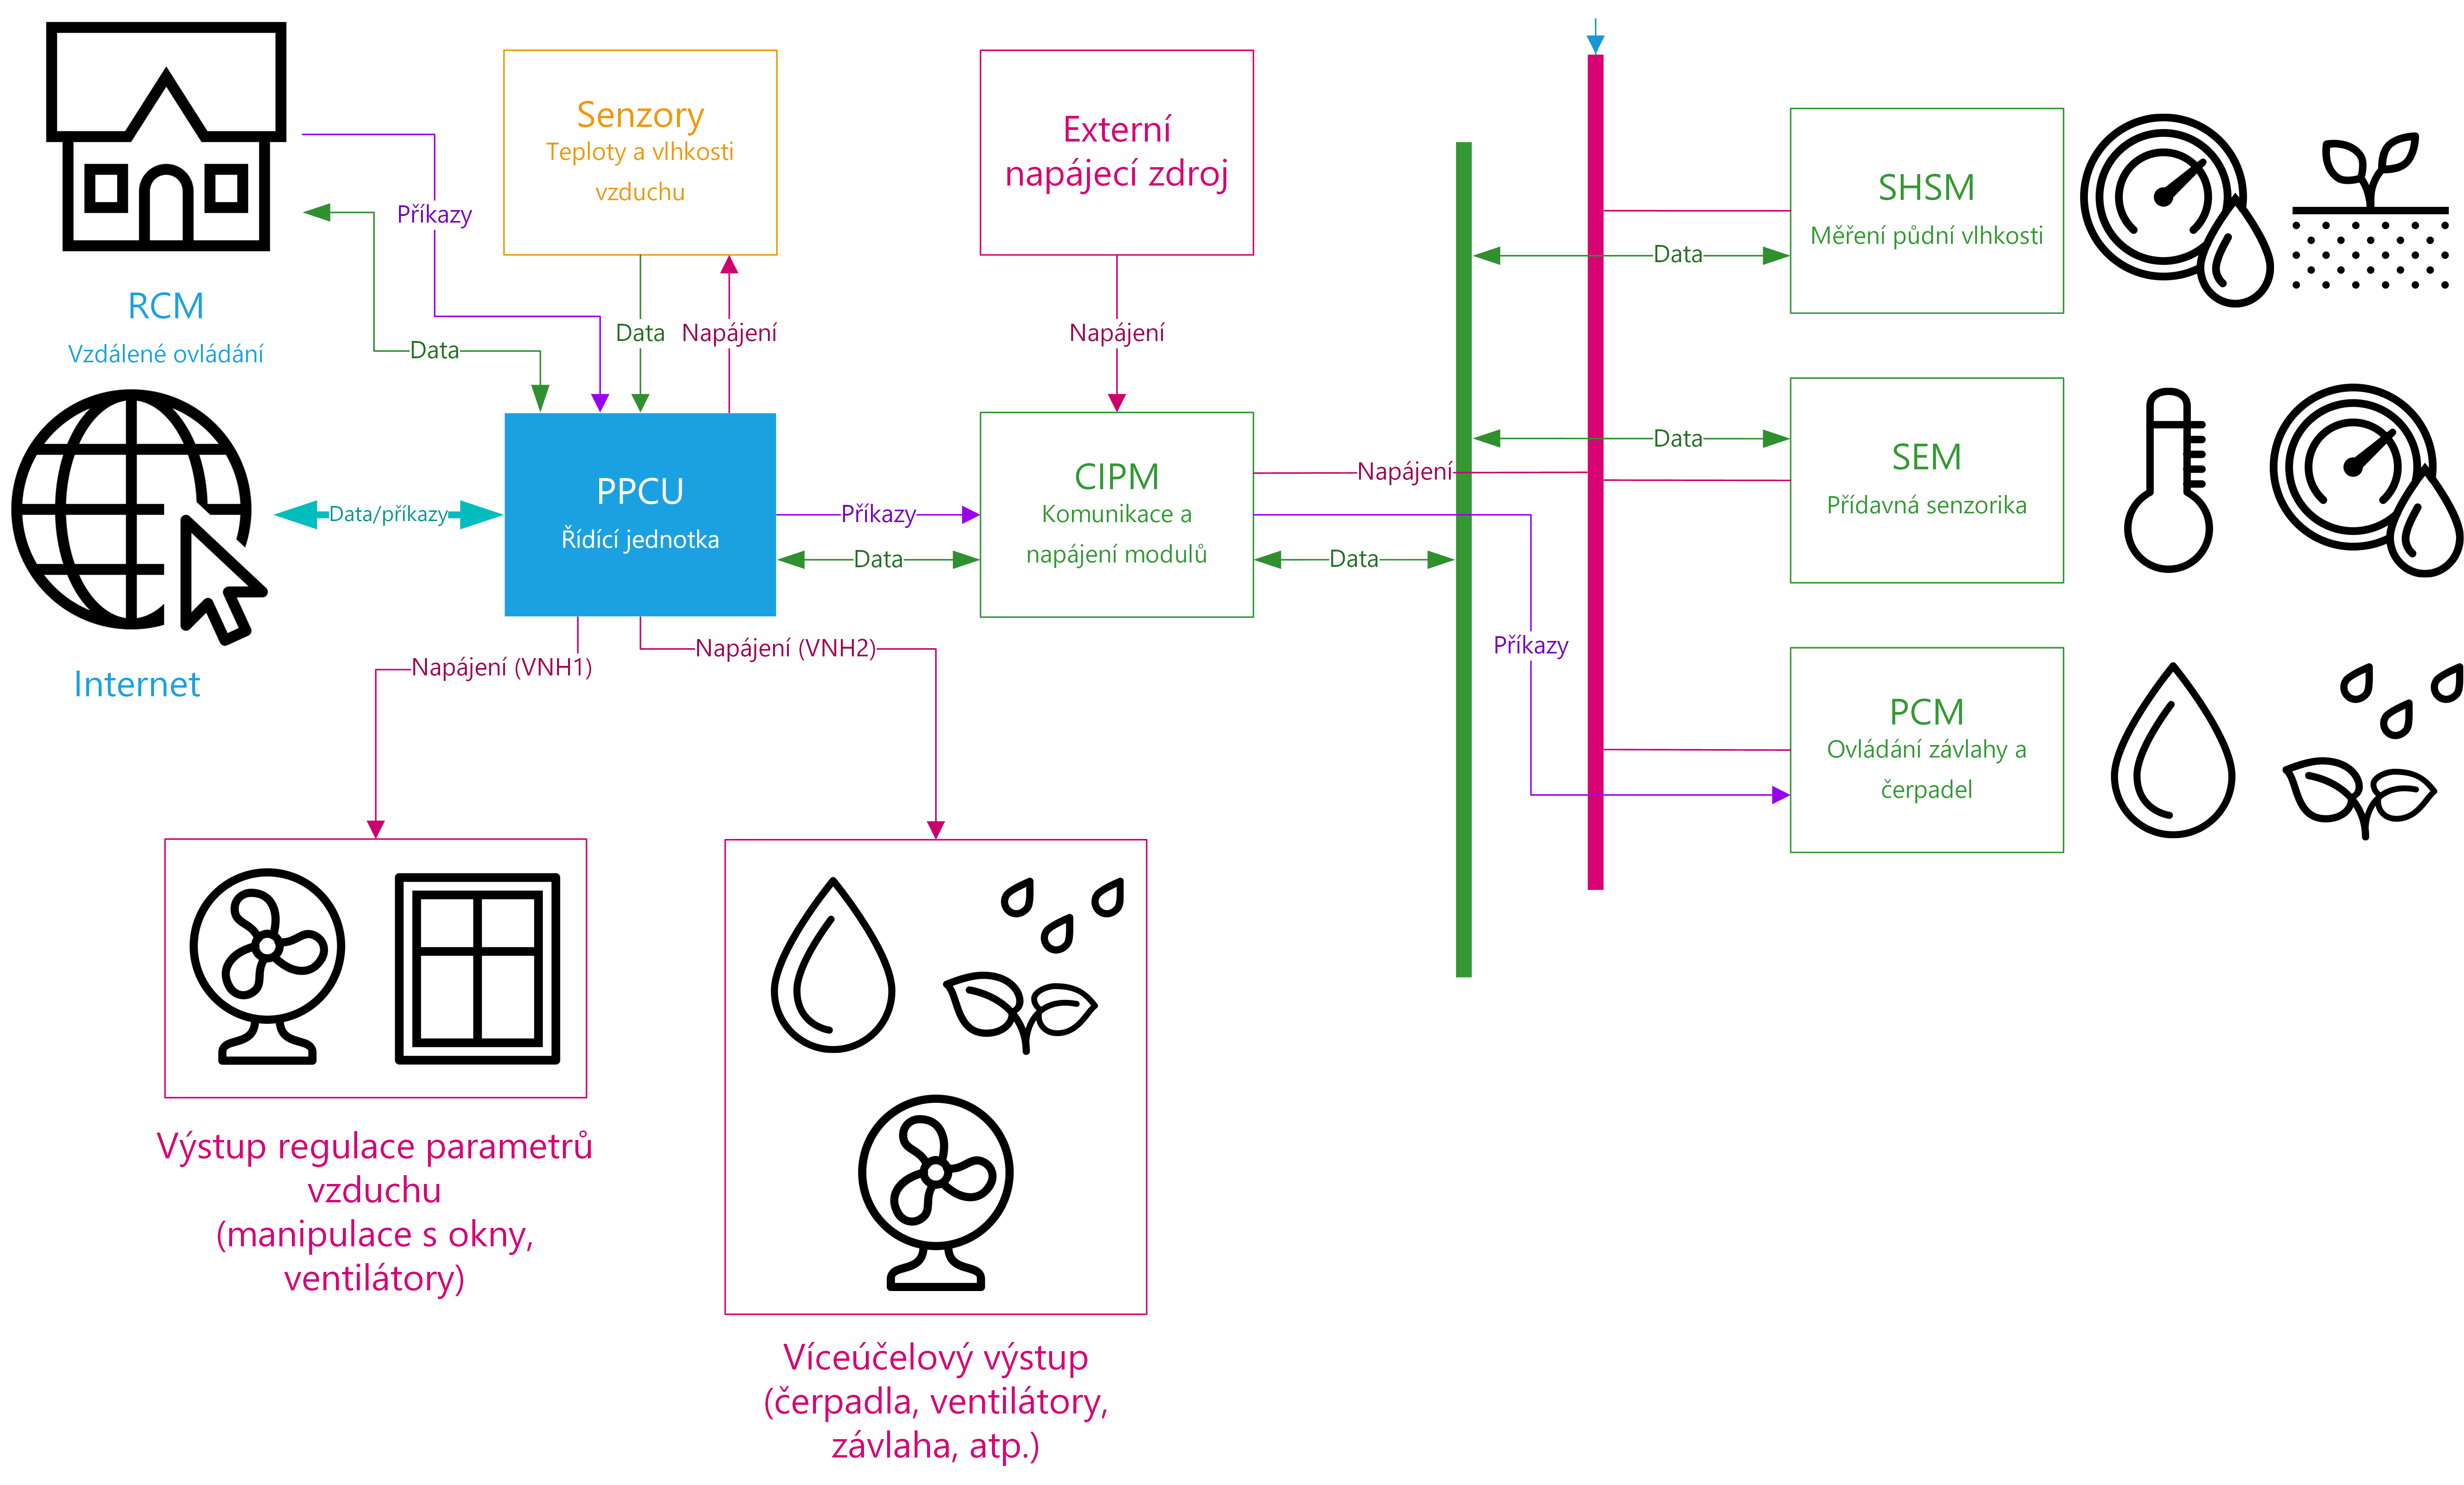
\includegraphics[angle=90,origin=c,scale=0.7]{img/HARDWARE/MODULES.png}
    \caption{Schéma zapojení a~funkce jednotlivých modulů.}
    \label{fig:add-MODULES}
 \end{figure}

\begin{figure}[h]
    \centering
    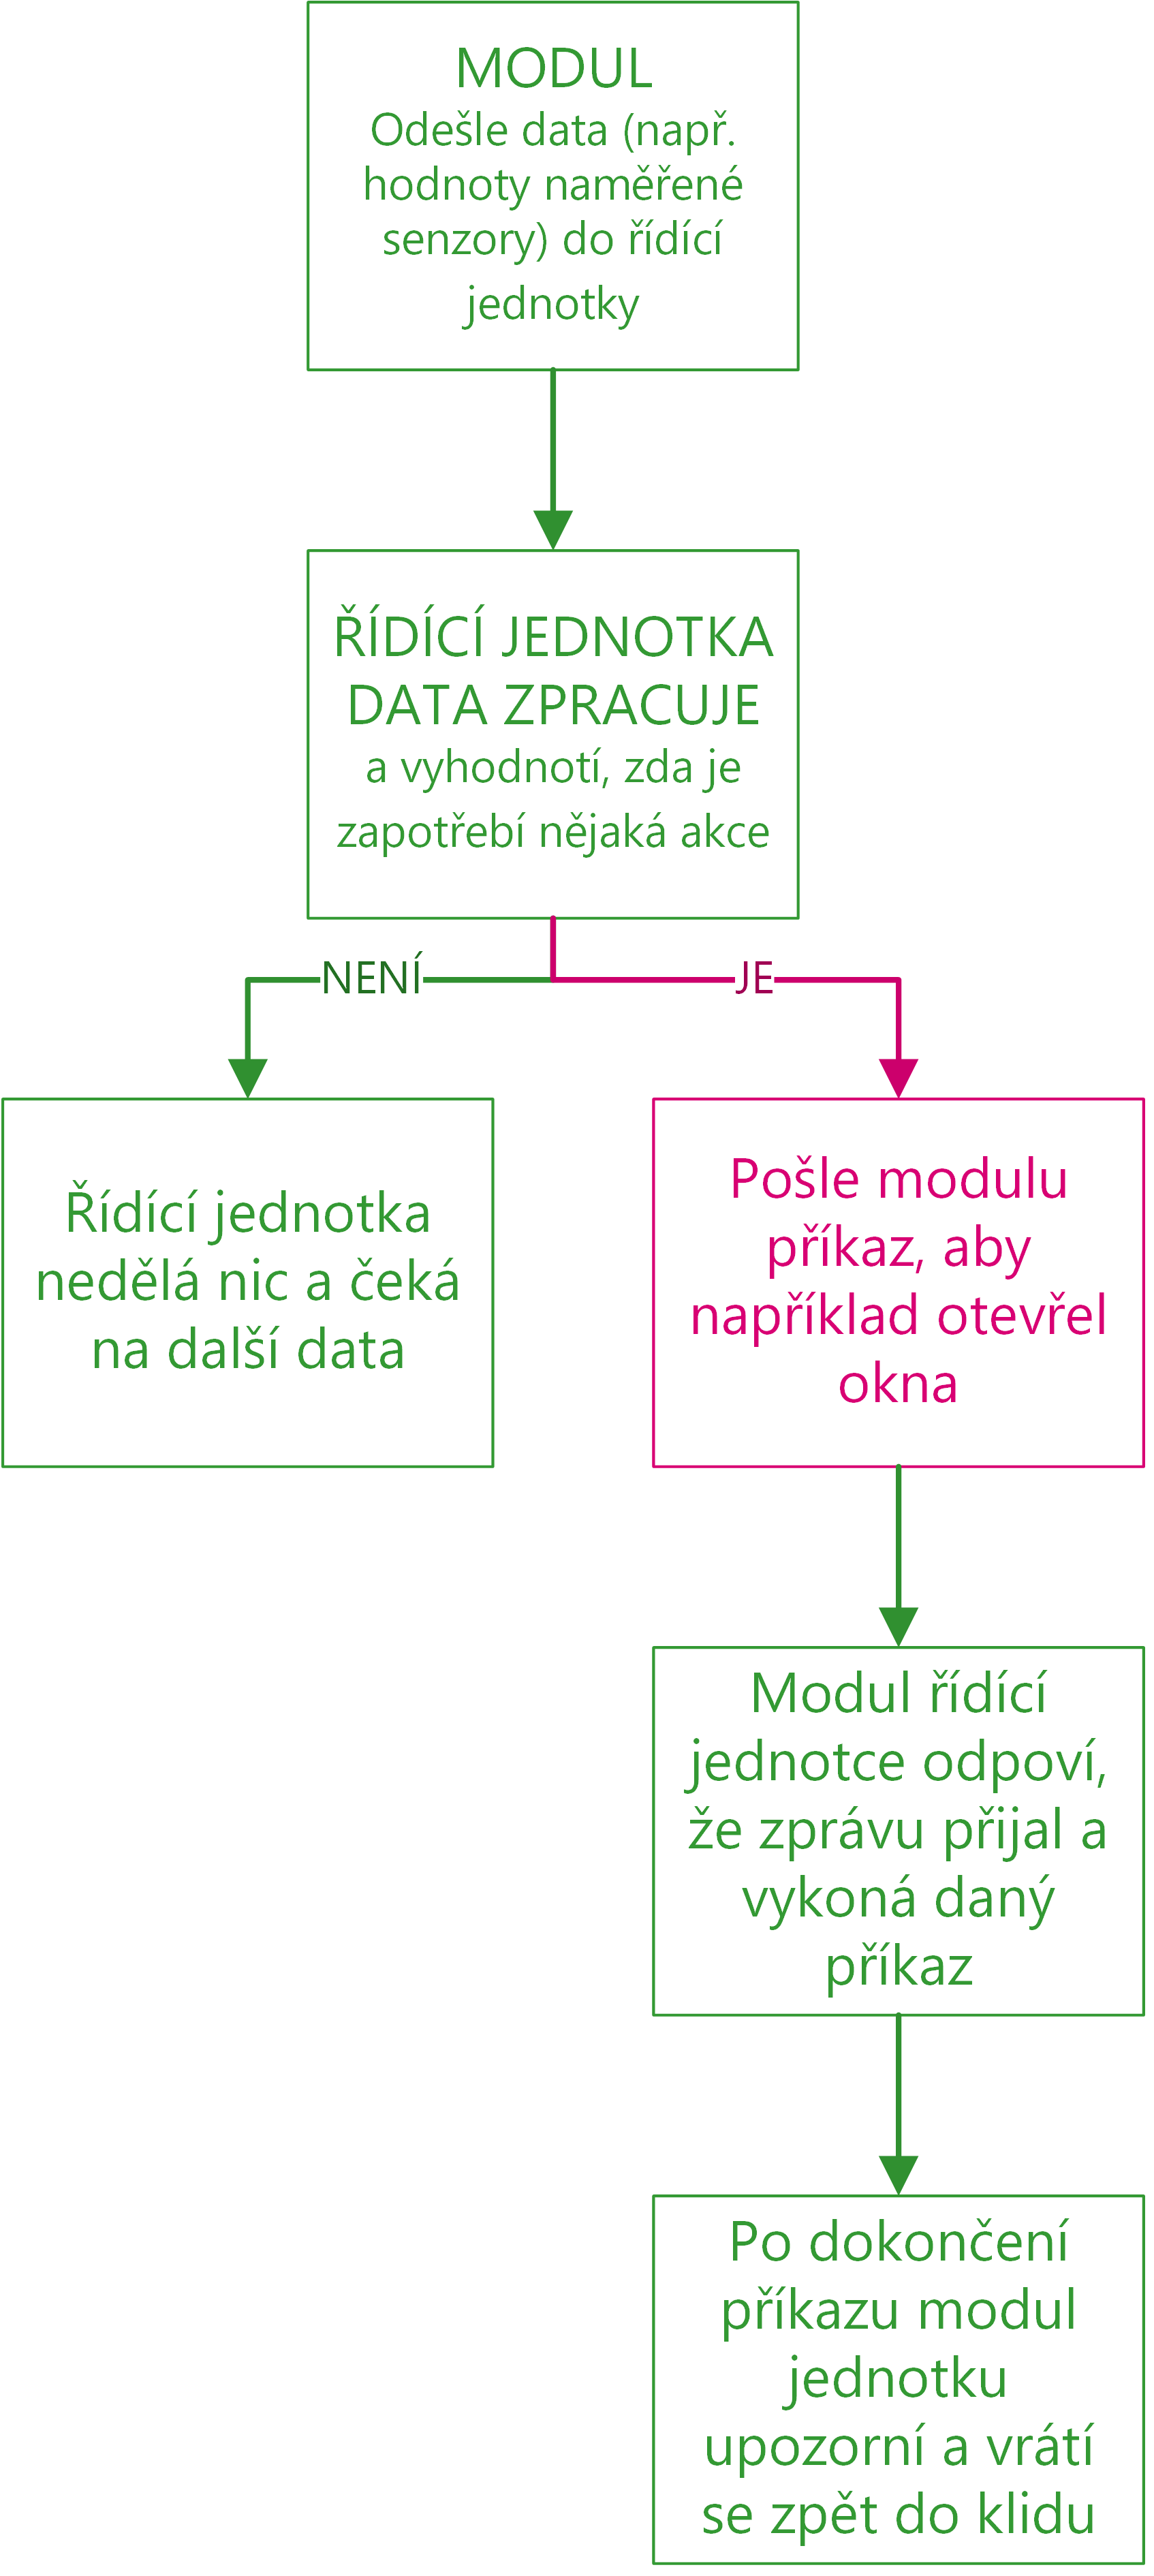
\includegraphics[scale=0.9]{img/SOFTWARE/KOMUNIKACE_MODULU.png}
    \caption{Blokový diagram komunikace řídící jednotky a~přídavného modulu.}
    \label{fig:PPCU-to-MODULE-communication}
\end{figure}

Stejným způsobem lze sázet další obrazové přílohy.
\newpage